%Points to be discussed:
%p1- Exponential evolution of networks, connectivity and telecommunication
%p2- The increase load and demand to fulfill daily tasks locally and remotely
%p3- Human body physical limitations
%p4- Need of enhancements to increase the efficiency of our tasks and remote operation
%p5- Advantages of digitization and overcoming the physical limitations
%p6- The possibilities of using digital media to customize our perception and leverage it with it
%p7- Why using remote avatars is better than direct wearable augmentations, and when
%p8- Propose Multi Scale Presence research concept, using digital media and remote avatars to enhance human, physically and perceptually

% Perception Overload: vast amount of information is presented to the user at once, which human can't perceive simultaneously.
% Human Augmentation: cognitive and physical improvements as an integral part of the human body


% Embodied Driven Design (EDD): Allow to customize body senses and actuators using Mediated Representation (Avatar) 

\chapter{Introduction}
\label{ch:intro}
\markboth{Introduction}{}

\begin{flushright}


\textit{``Before paper, wires, and silicon, the primordial communication medium is the body. At the
center of all communication rests the body, the fleshy gateway to the mind.``} 
\par\hfill\textsc{Frank Biocca, The Cyborg's Dilemma 1997}


\end{flushright}
\vspace{15pt}


We, as human beings or Homo sapiens, have evolved through a long adaptation process both our physical and cognitive abilities to fit into our environment and to achieve highly complex tasks using our bodies. Although compared to other biological animals, our bodies still considered quite limited in terms of sensory feedback. For example, we can not see or hear as well as other hunting animals due to the limited visual \& auditory spectrum, neither we can fly or dive in the sea same as other mammals can do. What was the edge that not only made us survive but also to be the superior race on earth? It is basically the use of tools and other mediums to overcome our biological limitations and to give us an edge both physically and mentally. Using the tools, our boundaries were not limited anymore to the skin, or the reach of the hand, but rather it created an extension to our physical bodies. Furthermore, when digital tools and means has emerged at our disposal, and integrated into our daily routine, the boundaries of our world has extended beyond the skull and the sight of our eyes. The digital era created radical changes in our cognitive skills, and changed how we manage our work and daily social activities. %Adding to that, the advancements in miniaturizing computational chipsets, sensors, and actuators has opened the door for direct body augmentation and the usage of wearable devices to assist our daily tasks in a ubiquitous and a seamless manner, or being used to recover a limitation of our bodies.

\section{Radical Bodies}

The role of tools has effected our adaptation to our environment, and created radical means to our body functions. The use of technological means can be generally divided into two application categories: supportive, and augmentative. The first category, supportive applications domain, is mainly concerned with recovering certain body modality disability (such as a lost limb, poor vision), while the second category, augmentative applications, is used to expand what a healthy and functional body modality can do (such as providing digital information to our vision modality). These two categories are illustrated in \Figure{fig:intro-radicalbodies}. Both categories falls under what is referred into as ``Radical Bodies'', that is the use of tools and devices along our biological body to overcome what can be considered as a limitation, or leveraging certain functions, and thus changing the behaviour of our bodies radically. 

\begin{figure}[b!]
  \centering
  \includegraphics[width=1\linewidth]{figures/intro/RadicalBodies.pdf}
  \captionsetup{justification=centering}
  \caption{Radical Bodies, and the proposed Embodied-Driven Design (EDD) approach position.}
  \label{fig:intro-radicalbodies}
\end{figure}

Supportive tools help the physically disabled community to regain their lost functions and to assist them in engaging in their daily and social activities in an independent manner. According to the American Community Survey (ACS) \cite{disabilities2016}, an estimation of 12.6\% of the overall population in the United States suffers from a physical disability in 2015. The physical disability is varied as a hearing, vision, cognitive, ambulatory, self-care, and independent living. Also, the survey showed that the rates of disability increase with age. From the entire US population, for working class with ages of 18-64, the rate was 10.5\% (contributing to 51.1\% of the disabled community), while for elder people with ages of 65 and above the rate was 35.4\% (contributing to 41.2\% of the disabled community). The body inherited functions (non-cognitive) showed to be the highest factors to the disabilities. Tools for this category of users are described as Assistive and Adaptive technologies \cite{Tennessee2012standards}. Assistive Technology is any object or system that increase, maintain, or improve functional capabilities of individuals with disabilities (such as glasses, hearing aids, ...etc), while an Adaptive Technology is any object or system that is specifically designed for the purpose of increasing or maintaining the capabilities of people with disabilities and seldom to be used by non-disabled persons (such as wheelchairs, white cane, ...etc). That is, assistive technologies are the wider umbrella that adaptive technologies are a subset of. Adaptive tools usually require the disabled person to adapt to its new function and to train his cognitive skills to substitute his lost function ( a blind person needs to adapt to the limits and range of his white cane, as it will become his eyes). Thus it can be seen that our bodies (disabled or functional) have the capacity and plasticity to adapt to new representations of its functions. It is, however, the adaptation process is variant depending on the design and interaction with the substitution device or tool. If the user is required to maintain constant awareness toward the device used (through his various perceptual modalities), then the device is considered as a foreign object which does not function as an embodiment of his action.

Augmentative tools on the other hand leverage the functions of the human body, and allows to extend and expand beyond the inherited biological limitations. Augmentation technologies can be categorized into two classes: invasive and wearable (non-invasive). Each set of these two classes has its own merits as well as its disadvantages physically, socially, technically,..etc. As an example of the earliest trials on direct body implants of electronic devices other than for medical purposes, in 1998 professor Kevin Warwick implanted a radio transmitter into his left arm which communicates with computers to open doors whenever he approaches them. Interestingly, after nine days of using it, he reported the implant felt as being part of his body \cite{warwick2000cyborg}. Although this experiment can be seen as naive (a wearable device can serve the same purpose), but it was one of the initial trials of radical bodies changes, and has a future of transcending our bodies via the combination of biological and technological means. However, one of the major disadvantages of such augmentation is the high cost of replacement and upgrades both physical wise (need for a surgery, the risk of infections) and money wise (the cost for that surgery). Such augmentations are still immature technological wise, and widely unacceptable socially. The other set of augmentation, non-invasive type, had a better success at proving that our bodies can be altered safely and at rather low costs. This set has existed as far as the glasses were used to enhance poor vision. Neil Harbisson \cite{harbisson2012listen} used this type of wearable devices to overcome his color blindness by using a head-mounted camera which translates colors into sound frequency, and after adequate usage of it his perception adapted to this new perception. Current wearable technologies even provide a way to alternate our perception and realities. A \textbf{perceptual proxy} device, such as Virtual Reality (VR) Head Mounted Display (HMD), headphones, or tactile actuators, under certain conditions, can deliver sufficient information to sensory organs to convince the brain of the new reality. The idea of altering and augmenting our bodies has been a driving force for various technologies and media we use on a daily basis. This wave produced a constant hype towards human-centered technologies. A visible trend in empowering technologies can be seen by Gartner's review of emerging technologies hype cycle of the year 2016 \cite{hype2016gartner} in \Figure{fig:intro-hype}. Virtual Reality and Augmented Reality have already become mature enough for the end user's application due to the long history of trials and applications \cite{rheingold1991virtual}. However, Human Augmentation is still an emerging topic with high expectations for enhancing and empowering our bodies instead of just being a supportive hardware or for rehabilitation purposes. This topic is still in its infancy and requires further philosophical approaches and scientific experiments to evaluate its effectiveness. 

\begin{shaded}
\footnotesize
\centering
\textit{Radical Bodies are the result of the technological integration with our bodies, leveraging our physical constraints and enabling wider set of embodied functions.} 

\end{shaded}

\begin{figure}[t!]
  \centering
  \includegraphics[width=0.9\linewidth]{figures/intro/gartner_hypecycle2016.pdf}
  \captionsetup{justification=centering}
  \caption[Gartner's Hype Cycle for Emerging Technologies 2016]{Expectations of human centered technologies. Gartner's Hype Cycle for Emerging Technologies 2016 (Modified from source for formatting purpose).}
  \label{fig:intro-hype}
\end{figure}

These tools and technological means have influenced radical changes to our perception and levitated our physical/mental abilities exponentially. The radical changes do not have to refer to the physical alteration of the human body (or mutations), but rather to how we act and communicate with the environment surrounding us. For example, today's advancement in the digital communication enabled us to overcome the spatial and temporal constraints. Internet-connected smartphones which are being used on a daily basis, have created radical changes in our social activities. A user communicating through it with a remote person is referred to be ``here'' and ``there'' at the same time. ``Here'' is where his physical body is located at which uses the smartphone to type and watch, while ``there'' is where a part of his cognition and awareness is actually at. Furthermore, virtual reality tools can carry the entire sense of presence and awareness into a totally different space or reality, in which the human body is no longer constrained by any physical limitations. The physical body is no longer defining the action, rather is being the medium between the internal intention and where the action is being performed. The more these technologies are integrated to our daily routine and appliances, the further the radical changes will be reflected on our bodies, and the more our biological bodies will be transparent in the process (mediums of actions). What if its possible to think of the body as being just a medium? Is possible to redefine this medium or ``rewire'' methodically? How to maintain this newly defined medium as being part of the body, or being the new body? In this thesis I address these questions by proposing the idea of ``Embodied-Driven Design (EDD)'', the use of body functions and modalities abstraction to allow us to redesign the functionality and the mapping of the body while maintaining the sense of ownership toward it.  \Figure{fig:intro-radicalbodies} shows the position of Embodied-Driven Design as an approach to establish a binding between our biological bodies and technologies in order to over come a physical disability or a limitation inherited within our bodies. EDD establishes an abstract modeling approach in order to reconfigure our bodies with an alternative representations, thus altering the embodied actions and cognition using mediated technology.

%To support this transition, or the integration between biological bodies and artificial means, a major research area ``Augmented Human'' has been established to leverage the human bodies capabilities using mediated tools.

%\subsection{The Hype of Human Augmentation}

\pagebreak
\section{\ProposalKeyword}% Metapresence

%\textit{\textbf{``Meta'': Abstraction} referring to a high level design approach.}

%\updatedtext


In this section, an overview of the thesis is described, the motivation and concept progression, along with the proposed approach addressing the thesis statement. 

\subsection{Thesis Statement}

In this thesis, I discuss the possibility to re-configure our bodies in a way that can alter our cognitive abilities or overcome our innate limitations and physical disabilities using mediated representations. With such re-configurations and alterations of our body schema, we can look at the use of the representations (for example technological tools) as being part of our bodies, embodied in a way we interact through them instead of using them. This sort of embodiment can establish a new form of interaction loop between our bodies and the environment (locally or in a different location), that our cognition is shifted into the active performance of intended actions instead of how we use the tools to achieve such actions. The relationship between body and action is mediated through embodied means of interactions and representations. This shift of perspective in using tools and technology would create an impact on how we perceive through and act within the environment in a way our bodies become actively part of it through our mediated and embodied actions. 

%Here I propose an Embodied-Driven Design approach for altering the body mapping, and focuses on the body transfer model in which it defines the relationship between the human body and the representation used. This approach is concerned with the flow of the body actions and sensory feedback, and it defines the interaction loop of the body model with its representation(s). Both the transfer model and the representation are the actual realization of the intended body schema model.

%Using this proposed approach, it is possible to adapt to new body forms which are considered driven from our embodied behaviours. 



\subsection{Motivation \& Approach}

The capability of remapping our exteroceptive modalities (visual, auditory, tactile, taste, and smell), and proprioceptive modalities such as body and joints posture with an alternative body representation can help to levitate the upper bounds of our physical limits. For example, for a true ubiquitous presence a person should be capable of receiving inputs from multiple locations simultaneously, thus we can say this person is ubiquitous as being in everywhere. His body and sensory modalities are not ``physically'' there, but his perception of these modalities is linked to them, and body sensory flow has became altered and remapped. Other topics can also be achieved, such as expanding the localization of body parts from being tightly coupled in one location (on the body) into being loosely coupled and distributed in multiple locations. Adding to that, body representation does not have to be tangible as long as it serves the application intended to, for example when the body is needed to represent the visual appearance of the user or the state the user is at, then it's sufficient to use a non-physical representation for that purpose. In these terms, the concept of body stretches from a tight physical representation which its parts are coupled spatially and tangibly, into loose physical/virtual representations that can be restructured and remapped. This expansion would provide new forms of awareness alterations and perception enhancements. Indeed there are issues that might arise when new forms of perceptual augmentation occur which we are not adapted to, such as perception overload (when several information sources are provided into the same perceptual modality, such as eyes or ears), or non-intuitive interaction is being used (not correlated with body motion, and requires training to learn it). 

In this thesis, I argue that the human body schema can be altered and adapt to new forms of body structures as long as the actions mapped between the body and its new representation are correlated. \ProposalKeyword conceptualizes the idea of using digital media and mediated technologies to alter human body properties on a high and abstract level, achieving new ways to transcend our perception and body capabilities. This approach addresses both local and remote body mapping, expanding the human spatial reach and reducing the physical constraints. \ProposalKeyword derives from the school of philosophical thought named as ``phenomenology'', which is concerned with how we perceive, experience, and act in the environment surrounding us using our body. Further details regarding the philosophical background of this research will be discussed in \Chapter{ch:related}. 

\subsection{Concept Development}

The human body is the interface of the mind, the medium to the tangible world and the embodiment of our thoughts. Its where the action is performed at and its the bridge which connects our world too, what we may say our self. My research and background in Telexistence area had inspired me to focus more on the possibilities to use mediated technology to expand our body instead of just replicating it. How to create a model of the human body that enables us to extend, enhance, and modulate our embodied functions was and still the driving force of \ProposalKeyword. I believe that in order to come up with such a model, an abstraction of the human body is needed that provides a systematic approach to embodied modeling.

This thesis investigates toward an abstraction model of the human body that enables us to redefine the actions and affordabilities which our cognition can represent. Our bodies constitute physical limitations, while the inner mental model of the body is far more adaptable to variations and reconfigurations. This work shows the possibility to rewire (or reprogram) the body in order to overcome an existing physical disability or to leverage the capacity of human body perceptual \& postural limitations. These arguments are supported by philosophical background research and empirical studies that build up the concept of \ProposalKeyword.

The idea behind \ProposalKeyword was developed across several projects and iterations which helped me to generalize the idea of meta-modeling, and the design of body schema transfer systems. Along these iterations, four different meta-modeling approaches were developed and used to address body limitations and physical disabilities. These meta-modeling approaches were used in five projects. These iterations along with the projects that involved in each of them are illustrated in \Figure{fig:intro-progression} with the corresponding projects that address. 

The first design iteration \textit{Direct Body Transfer} was initiated based on my involvement in Telexistence area of research since 2013. This approach develops the concept of mapping our body's functions and modalities directly into a corresponding representation without the need of alteration or modifications. Such mapping pattern is useful to transfer body parts directly from one location to another. Telexistence type of systems uses such pattern to copy user's body motion into a remotely connected avatar system, and replicate the feedback back to user's body. ``Telexistence based Surveillance System'' project in the period of 2014-2016 (\Section{sec:eval-txSys}) mainly uses this design approach to overcome body spatial limitations.

%This approach basically contributes at the type of systems that overcomes spatial constraints in teleoperation applications. My involvement in ``Telexistence based Survellance System'' project in the period of 2014-2016 (\Section{sec:impact-txSys}) developed the necessary elements for providing direct and real-time body transfer systems. This approach has been incorporated as a basic building block for direct body transfer meta-modeling. 

\begin{figure}[t!]
  \centering
%	  \centerline{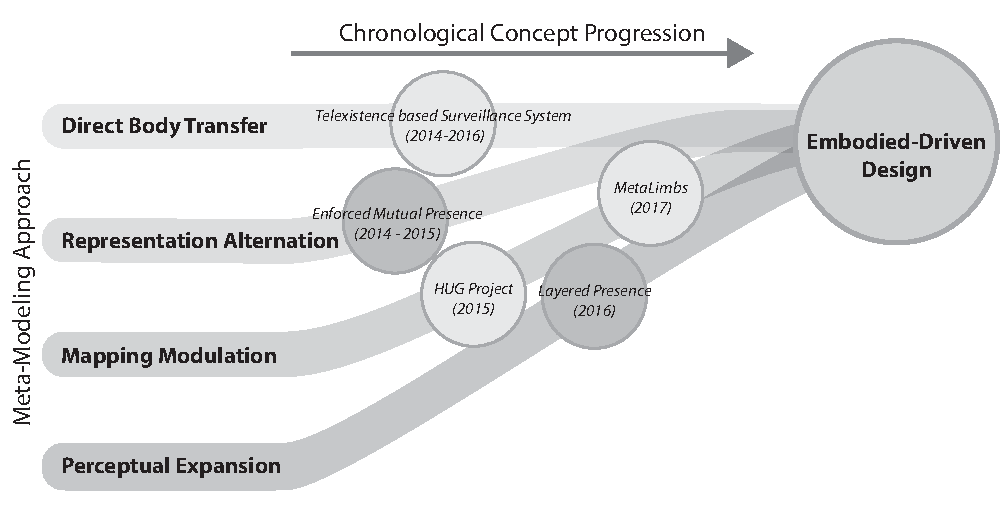
\includegraphics[width=1.2\linewidth]{figures/intro/ConceptProgression.pdf}}
	  \centerline{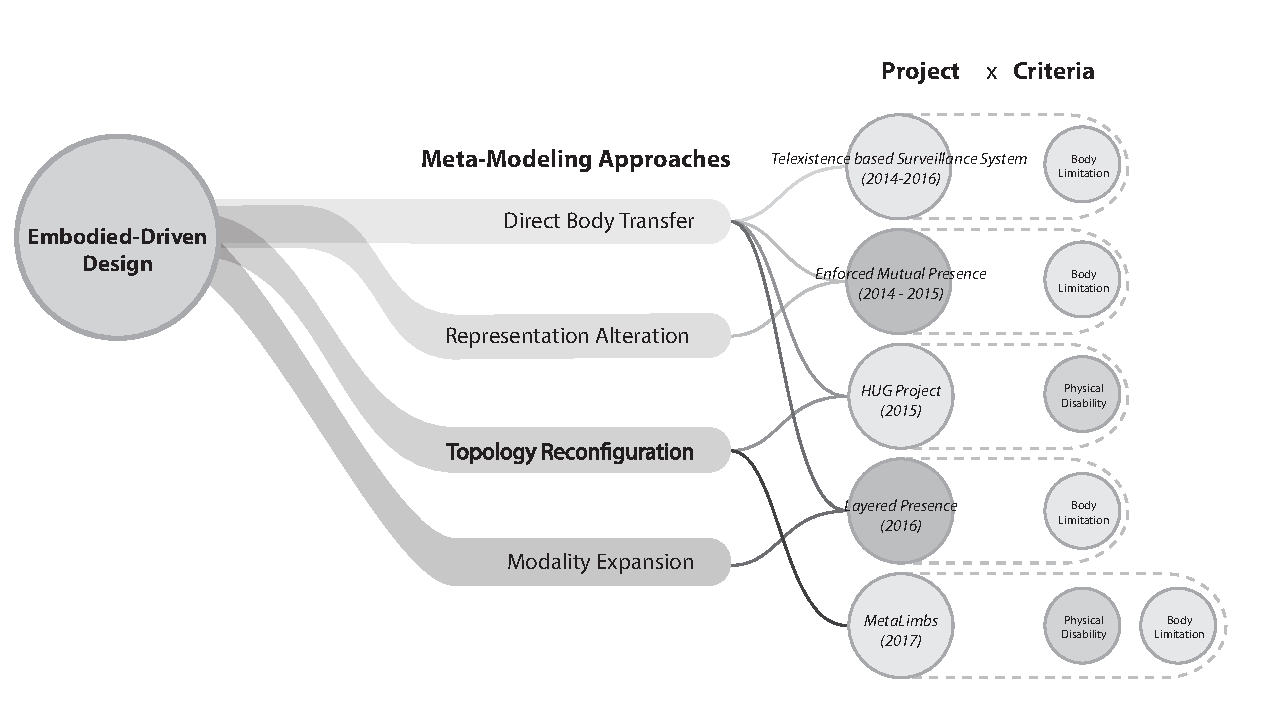
\includegraphics[width=1.2\linewidth]{figures/intro/MetaModelingOverview.pdf}}
  \captionsetup{justification=centering}
  \caption{The use of Embodied-Driven Design Meta-Modeling approaches to address five projects, highlights the need of such design approach to resolve body limitations and disabilities.}
  \label{fig:intro-progression}
\end{figure}

The second design iteration \textit{Representation Alteration} aims to overcome the physical limits constituted by our bodies. It combines a hybrid approach for altering the representation of our bodies using virtual and physical means. Thus the body is mediated through tangible and non-tangible representation overcoming certain physical limitations. ``Enforced Mutual Presence'' achieved in 2014-2015 (\Section{sec:eval-enforced}), explores the use of virtual representation along a physically teleoperated system to achieve a full sense of body presence despite the fact the system does not have a full physical body. Virtual hands substitute user's arms were projected locally and remotely at the teleoperated system. This substitution not only helped at providing the full awareness of the body, but also the use of non-physical hands helped to overcome the tangible constraints of arm's length limits. Thus the operator is capable to stretch his body across spatial space. With such alternative body representations, it is possible to design new body forms that overcome our bodies' physical limits (such as extending arm reach and pointing for mobility impaired people).

%This project helped at defining a meta-model for representation alteration, that is the use of a combination representations for the body. With such alternative body representations, it would become possible to design brand new radical forms which our physical bodies can not achieve.

%The use of direct body mapping means that the representation side is required to have same functions which the human body can link and map into, such as physical arms, hands, eyes, ...etc. However, in situations that the representation does not matches human body properties and topology, then 

%To overcome such a requirement, the second iteration was aimed to solve the physical body constraints by using hybrid body representations. Enforced Mutual Presence 2014-2015 (\Section{sec:eval-RepAlt}) explored the use of virtual contents along a physically teleoperated system to achieve full sense of body presence despite the fact the system does not have full physical body. The approach used is to use virtual hands driven from the user's body which are projected locally and remotely at the teleoperated system. This not only helped at providing the full awareness of the body, but also the use of non-physical hands visuals helped to overcome the tangible constraints of arms length limits. Thus the operator is capable to stretch the body across the spatial space. This project helped at defining a meta-model for representation alteration, that is the use of a combination representations for the body. With such alternative body representations, it would become possible to design brand new radical forms which our physical bodies can not achieve.

The third design iteration \textit{Topology Reconfiguration} explored the plasticity of human body operation mapping, mainly the postural mapping. Two projects helped in formulating this design approach: the first is ``HUG Project'' in 2015 (\Section{sec:eval-hug}) that used eye gaze input to control the head rotation of a remote system supporting a physically disabled person to operate it. The second project is ``MetaLimbs'' in 2017 (\Section{sec:eval-metalimbs}) that explored remapping body legs with artificial arms mounted on user body, thus expanding the number of independent arms. Both projects showed the immediate adaptation the body can achieve to a different mapping schema. This iteration established the design of body postural topology that is used as one of the foundations of this approach.

Last design approach explored is \textit{Modality Expansion} that addresses the possibility to expand the perceptual modalities of our body and the capacity to remap our sensory and postural topology to multiple representations simultaneously. ``Layered Presence'' in 2016 (\Section{sec:eval-layeredpresence}) studied this body schema and proposed a modeling approach to achieve such expanded spatial awareness. This project helped to shape the perceptual modalities mapping and an interaction model which helps in developing this approach.

These four iterations motivated the design of a meta-modeling approach for human body schema, and defined the foundations of the proposed modeling framework. \ProposalKeyword and its realization as a framework are aimed to assist designers and researchers in this field to prototype and deploy new forms of body schema.


%This work proposes a novel design approach for altering human perception mapping with remote avatar surrogates to achieve what is called ``\ProposalKeyword'' based on \textbf{Loosely-Coupled Modality} (LCM) design pattern, and using \textbf{Embodied-Driven Design} (EDD). Using this design concept, the perceptual representation combines both physical and virtual tools to define to reconstruct the relationship between our sensory organs and the corresponding inputs, and same wise for actuating organs. \Figure{fig:intro-evolvement} shows the differentiation between Telepresence and Telexistence in terms of design perspective. Metapresence covers the concepts in Telexistence, and adds an embodied driven design approach using meta prototyping tools. Further details follows in Chapter 3 about Metapresence design approach.

%      Further details follows in Section \ref{sec.EDD}.





%%%%%%%%%%%%%%%%%%%%%%%%%%%%%%%%%%%%%%%%%%%%%%%%%%%%%%%%%%%%%%%%%%%%%%%%%%%%%%%%%%%%%%%
\subsection{Research \& Design Topics:}


\Table{intro:research-topics} summarizes an overview of the topics that constructs the concept of \ProposalKeyword. Research and design topics addressed in this thesis outline body schema modeling approach.

The first part addressed is focused on the design approach for \ProposalKeyword and is discussed in \Chapter{ch:concept}. A framework is developed based on a systematic model of human body schema in which its possible to remap and restructure it hierarchically. It outlines the methodology to form a meta-modeling approach that realizes the proposed concept. EDD is constructed and designed based on the following topics:

\begin{enumerate}[label=T\arabic*.]
 \setlength\itemsep{0em}

\item \textbf{Loosely-Coupled Modalities (LCM):}

Possibility to decouple body modalities into a set of ``input/output channels'', and to re-couple them. The loosely representation helps to break the coupling of the physical modalities and constraints, and thus allows to achieve a higher level of mapping of the human body to its representation(s). LCM defines two topologies for the human body: Postural and Sensory. These topologies serve as generalization and abstraction for the postural modalities of the body (connection between the various body joints), and the sensory modalities. Further details are discussed in \Section{sec:concept-LCM}.

\item \textbf{Body Schema Meta-Modeling:}

Ability to remap our bodies modalities into new body schema. This topic argues that our body structure can be reconfigured or reprogrammed. The meta-models define the structure of the sensory and postural channels mapping between the human body and the corresponding representation(s)' modalities. In these models, transfer blocks are used to characterize the function and data flow between the modalities used. Further details are discussed in \Section{sec:concept-bodyschema}.

\item \textbf{Meta-Modeling Approaches:}
Four meta-modeling approaches are proposed that summarizes the general usability methods of EDD within this thesis, and which can be generalized for applications beyond what is discussed. The purpose of these approaches is to facilitate the design process, and to highlight how to address body limitations and disabilities using meta-modeling. Further details are discussed in \Section{sec:concept-metalmodel}.

\end{enumerate}


\begin{table}[t!]
\scriptsize
\centerline{
\begin{tabular}{lll}
\toprule
  \textbf{}    & \textbf{Category} & \textbf{Reference} \\ 
\midrule
\textbf{Topic} &    \textbf{Embodied-Driven Design}       &   \Chapter{ch:concept}   \\
\textbf{T1.} & Loosely-Coupled Modalities: Recon-structure body schema based on a hierarchical topology  &       \Section{sec:concept-LCM}     \\
\rowcolor[gray]{.9} 
\textbf{T2.} & Body Schema Meta-modeling: Abstraction of body modalities interaction and mapping  &   \Section{sec:concept-bodyschema}    \\ 
\textbf{T3.} & Meta-Modeling Approaches: Four design patterns for body schema editing &   \Section{sec:concept-metalmodel}    \\ 
\midrule
\textbf{Project} &    \textbf{Meta-Modeling Evaluation}        &  \Chapter{ch:eval}   \\
\textbf{P1.} & Telexistence base Surveillance System: Addressing spatial limitations & \Section{sec:eval-txSys}              \\
\rowcolor[gray]{.9} 
\textbf{P2.} &  Enforced Mutual Presence: Addressing body physical limitations & \Section{sec:eval-enforced}  \\ 
\textbf{P3.} &  HUG Project: Addressing body plasticity to overcome physical disability   &  \Section{sec:eval-hug}                \\ 
\rowcolor[gray]{.9} 
\textbf{P4.} &  Layered Presence: Addressing perceptual plasticity  & \Section{sec:eval-layeredpresence}  \\ 
\textbf{P5.} &  MetaLimbs: Addressing body plasticity and limbs limitations       &  \Section{sec:eval-metalimbs}                \\ 
\bottomrule
\end{tabular}
}

  \captionsetup{justification=centering}
\caption{Topics and projects addressed in this thesis to realize \ProposalKeyword. }
\label{intro:research-topics}
\end{table}



The second part of this thesis in \Chapter{ch:eval}, evaluates meta-modeling approaches through five different scenarios addressing human body limitations and/or physical disabilities. An overview of the main points addressed within these projects as follows:

\begin{enumerate}
 \setlength\itemsep{0em}
\item Spatial limitations: Expanding body spatial accessibility and awareness through mediated representations, which is mainly addressed through P1.``Telexistence base Surveillance System'' in \Section{sec:eval-txSys}.

\item Body physical limitations and disabilities: Possibility to use different body representation to overcome physical constraints, addressed through P2.``Enforced Mutual Presence'' in \Section{sec:eval-enforced}, P3.``HUG Project'' in \Section{sec:eval-hug},and P5.``MetaLimbs'' in \Section{sec:eval-metalimbs}.

\item Perceptual plasticity: Use of EDD to alter body modalities to expand the amount of perceptual feedback. P4.``Layered Presence'' in \Section{sec:eval-layeredpresence} illustrates visual perception plasticity into multiple remote locations.

\end{enumerate}

%\Figure{fig:intro-meta} highlights the differentiation between Telepresence and Telexistence design approaches, and highlights Metapresnce conceptual design.


%%%%%%%%%%%%%%%%%%%%%%%%%%%%%%%%%%%%%%%%%%%%%%%%%%%%%%%%%%%%%%%%%%%%%%%%%%%%%%%%%%%%%%%

\subsection{Summary of Contribution} 

The main contributions of this thesis can be categorized as follow:
\begin{itemize}

\item Conceptual Contribution: 

This thesis provides the building blocks for expanding and enriching the body augmentation area of research by connecting the theoretical studies and various questions in the philosophy of body ownership and metacognition with systematic methods for testing these theories. By providing a framework for body schema design and modalities alteration, it is possible to design and evaluate various models of body schema with an experience-oriented approach.
%evaluate and measure the degree of cognition and perception human can be aware of. 

\item Design and Implementation:

This thesis presents the design strategy of body schema meta-modeling based on four modeling categories: direct body transfer, representation alteration, topology reconfiguration, and modality expansion. These meta-models summarize the general design approaches which the body schema can be designed through. Each of these categories is addressed separately.

\item Social and Industrial Contributions:

During the course of this thesis, two projects in which the Embodied Driven Design (EDD) framework was used into. The first is ``HUG project'' in which EDD used as a social contribution, and ``Telexistence based Surveillance System'' as an industrial contribution.

\item Technical Contribution: 

Along the development of this work, various system optimization and technical details that assist the developers in telepresence/telexistence related applications were described in this thesis, such as \textit{Foveated Streaming}. These details are further discussed in \Chapter{ch:impl}.

\item Physical Embodiment Toolkit: 

As an outcome of this work, an embodiment toolkit has been designed and implemented. This toolkit provides essential functions for remote presence applications, and its functions have been integrated into the EDD framework as a set of representation modalities which can be accessed and mapped with user's body. This toolkit allows designers to use rapid prototyping and testing of their ideas along with the meta-editor.

\end{itemize}


\pagebreak
\section{Thesis Outline}

This research builds on the findings related to human body plasticity found in the areas of philosophy of body and perception, cognition science, and body augmentation. Also, it introduces the idea of \ProposalKeyword: altering body schema and sense of presence using a systematic and at a meta-level design. This thesis highlights the idea of digitized modalities -converting the biological/analog sensory and motor modalities into a digital representation- in order to overcome the inherited physical constraints and limitations. 
%By using the idea of digitized modalities, its possible to modify the perceptual information in a mediated environment in order to augment the human body. And with the ability to map and restructure body's functions into different schematics, it is possible to compensate a disabled function of the body by deriving its functionality from a different modalities, e.g. mapping a functioning limb into a disabled one.

%\end{itemize}


%\subsection{Meta-Modeling of Human Body}
%\pagebreak
%\section{Thesis Outline}

\subsection{Organization}

The core of this thesis is divided mainly into four parts and seven chapters organized as follows:

\begin{itemize}
\item \textbf{\Part{pt:I}: Foundations \& Philosophy}
\begin{itemize}[label={},leftmargin=*]
\item \textbf{\Chapter{ch:intro}.} provided the motivation behind this work, and briefly introduced the proposed concept: Embodied Driven Design.

\item \textbf{\Chapter{ch:related}.} explores the literature and philosophical background which Embodied-Driven Design is established on top of. Discusses topics related to Embodiment and Cognition that are regarded as the fundamentals of this research, and in which the idea of Embodied-Driven Design is placed within. It also provides several related work in human augmentation, presence alteration, and body representation which this research concept derives from, highlighting the contributions of this thesis.
\end{itemize}

\item \textbf{\Part{pt:II}: Embodied-Driven Design}
\begin{itemize}[label={},leftmargin=*]
\item \textbf{\Chapter{ch:concept}.} discusses in further details the proposed concept of embodiment design and the overall design considerations for an EDD framework, including the concept of loosely-coupled representation for human body. Four types of meta-modeling categories are described which summarize the design approaches of EDD: Direct body transfer, Representation alteration, Topology reconfiguration, and Modality expansion.

\item \textbf{\Chapter{ch:impl}.} provides the implementation process of EDD framework and meta-modeling editor environment, and describes in details the various building blocks for modeling body schema. The development of a physical toolkit is also discussed along EDD framework for general purpose presence embodiment.

\item \textbf{\Chapter{ch:eval}.} discusses five different projects and use-cases that highlights the role of EDD meta-modeling to resolve body limitations and physical disabilities. These study cases show the possibilities to modify our body schema to achieve new cognitive capabilities, such as expanding visual awareness and altering body limbs. 

\end{itemize}

\item \textbf{\Part{pt:IV}: Future Direction \& Conclusion}
\begin{itemize}[label={},leftmargin=*]
\item \textbf{\Chapter{ch:conc}.} concludes with a summary and reflections of this work, main contributions and outcomes, limitations, and finally presents an outlook for this research future direction. %, the limitations, and future direction to expand the topic of embodiment design and Metapresence applications.

\end{itemize}
\end{itemize}

\pagebreak
\section{Glossary}

The following keywords are described in the context of this thesis:

\begin{itemize}
\item \textbf{Agency}

Motor skill control, including the subjective experience of control, intention, sensory-motor selection and the conscious experience of will. Further details about the topic \cite{roessler2003agency}.

\item \textbf{Body Schema}

The mental model or self-image of the body, a subjective experience obtained through the cycle of operation and sensory feedback to create the global structure of one's perceived body.

\item \textbf{Embodiment}

The subjective experience of 'having and using' a body which interacts with the external surroundings, and reflects the inner intentions in correlation with cross-modal perception. The act of embodiment alters the mental image of body schema.

\item \textbf{Loosely-Coupled Modalities}

The possibility to decouple body modalities into a set of ``input/output channels'', and to re-couple them. The loosely representations help to break the rigid constraints of the physical modalities, and map body modalities separately.

\item \textbf{Meta-Modeling}

The process of defining an abstract model for the relationships between the various body modalities provided with an artificial representation's modalities.

\item \textbf{Modality}

In this thesis, a modality refers to a functionality derived from the human body or an artificial representation. The functionality can be described as an input if its related to the sensory feedback of the body, and an output if its related to an action can be performed by the body, such as joints motion.

\item \textbf{Ownership}

A reflected experience of identification a body as being owned by one's self (phenomenally experienced as 'mine-ness').

\item \textbf{Perceptual Proxy}

A device used to deliver/receive information to sensory/from actuating organs to induce a new sense of reality or to capture the structure of the body. Such as virtual reality equipment, haptic feedback interfaces, postural tracking devices.

\item \textbf{Radical Bodies}

The concept proposed in this thesis reflecting the radical changes of technology progression on human bodies in terms of interaction and perception within an individual or social contexts.

\item \textbf{Representation}

In this thesis, representation refers to the physical or virtual form of the modalities which can act as an extension or replacement of certain human body modalities. % (the relationship is defined by the meta-model)

\end{itemize}


%\footnotesize
%\bibliographystyle{dependencies/acm-sigchi}
%\bibliography{y-bibilography}